\chapter{\texorpdfstring{Measuring the CP structure of the Higgs-tau Yukawa coupling in $\PGt_h \PGt_h$ decays}{Measurement of the CP structure of the Higgs-tau Yukawa coupling in tauh tauh decays}}
\chaptermark{\texorpdfstring{Measurement of Higgs CP structure in $H \to \PGt_h \PGt_h$ decays}{Measurement of Higgs CP structure in H to tauh tauh decays}}
\thispagestyle{plain}  % First page has default style
\pagestyle{chapterpages}
\label{Section:Chapter_CP}
\minitoc

\section{Introduction}

As outlined in Section~\ref{Section:Chapter2_CP_Yukawa_Structure}, the CP structure of the Higgs-tau Yukawa coupling can be probed through spin correlations in $H \to \tau\tau$ decays. These correlations are captured in the acoplanarity angle $\phi_{CP}$ between the $\tau^+$ and $\tau^-$ decay planes, which serves as the primary CP-sensitive observable.

In the \ac{SM}, this measurement is expressed in terms of the effective CP mixing angle $\alpha^{\PH\tau\tau}$ (defined in Section~\ref{Section:Chapter2_HiggsCPStructurethroughHttdecays}), predicted to be essentially zero for a purely CP-even interaction. A significant deviation of $\alpha^{\PH\tau\tau}$ from zero would be direct evidence for CP violation in the Higgs–fermion sector, with important implications for physics beyond the \ac{SM}. Minimal supersymmetric models predict only negligible CP-violating effects in Yukawa couplings, whereas extended Higgs sectors such as the next-to-minimal supersymmetric model can accommodate values up to ${\sim}27^\circ$~\cite{King:2015oxa}.

The most precise determination to date was performed by the \ac{CMS} Collaboration using the full Run 2 dataset of $137~\mathrm{fb}^{-1}$ at $\sqrt{s} = 13~\mathrm{TeV}$~\cite{HiggsCP_CMS_2021}. That analysis combined multiple $\tau$ decay channels, including leptonic modes ($\tau_e^\pm,\ \tau_\mu^\pm$) and the dominant hadronic modes ($\pi^\pm$, $\rho^\pm \to \pi^\pm \pi^0$, $a_1^\pm \to \pi^\pm \pi^0 \pi^0$, $a_1^\pm \to \pi^\pm \pi^\mp \pi^\pm$). The result, $\alpha^{\PH\tau\tau} = -1 \pm 19^\circ$, compared to an expected $0 \pm 21^\circ$ at the 68.3\% CL, disfavouring the pure CP-odd scenario at $3.0\sigma$, was dominated by statistical uncertainty. Feasibility studies indicate that a precision of ${\sim}5$-$10^\circ$ could be achieved with $3\unit{ab}^{-1}$ of data~\cite{Harnik:2013aja,Berge:2014sra}.

This chapter presents a complementary measurement targeting only the $\PGt_h \PGt_h$ final state. The dataset corresponds to the partial Run 3 data-taking period and is substantially smaller in integrated luminosity than in Run 2, leading to reduced statistical reach. Despite the smaller dataset, this analysis aims to approach the precision of the Run 2 results by targeting improvements in key components such as:

\begin{enumerate}[label=(\roman*)]
    \item Tau identification
    \item Triggering
    \item Tau \ac{DM} classification
    \item Event Categorisation
    \item Reconstruction of the sensitive observable
\end{enumerate}

These developments are aimed at paving the way to a competitive measurement well before the \ac{HL}-\ac{LHC} era, and will be discussed in more detail throughout this chapter, along with an improved analysis strategy.

\section{Collision data}

This analysis uses proton–proton collision data recorded by the \ac{CMS} detector during the initial part of the Run 3 period (2022–2023). The collisions were produced at a centre-of-mass energy of $\sqrt{s} = 13.6\TeV$, and the dataset corresponds to an integrated luminosity of about $61.9\unit{fb}^{-1}$.

\section{Backgrounds}
\label{Section:Chapter7_Backgrounds}

Many of the background processes relevant to the fully hadronic ditau ($\PGt_h\PGt_h$) final state are the same as those discussed for the four-tau analysis in Section~\ref{Section:Chapter6_Backgrounds}. The main difference is that the present selection requires only two reconstructed tau candidates, both hadronically decaying. Events can enter the signal region through three main mechanisms:  

\begin{enumerate}[label=(\roman*)]
    \item Production of two genuine $\PGt_h$ leptons  
    \item Production of one genuine $\PGt_h$ and one misidentified object (jet or prompt electron/muon reconstructed) as $\PGt_h$
    \item Production of two misidentified objects, typically jets or nonprompt electrons/muons, both reconstructed as $\PGt_h$
\end{enumerate}

Relative to the four-tau case, the composition and ranking of backgrounds change noticeably.  \textbf{\ac{DY}} ($\PZ/\gamma^*\to\PGt^+\PGt^-$) with both taus decaying hadronically is now the dominant source of genuine $\PGt_h\PGt_h$ pairs. \textbf{Top-quark pair production} ($\ttbar$) also makes a large contribution, both through $\PW\to\PGt\nu_\PGt$ decays (genuine $\PGt_h$) and through the misidentification of jets or prompt leptons as $\PGt_h$, with the associated $b$-jets increasing the likelihood of additional jet activity. Backgrounds from \textbf{$\PW$+jets} and \textbf{\ac{QCD}-induced multijet production} are similarly important, as only one or two jet$\to\PGt_h$ (or $e/\mu\to\PGt_h$) misidentifications are needed to pass the $\PGt_h\PGt_h$ selection.  

In contrast to the four-tau analysis, where \textbf{$ZZ\to4\PGt$} was the most important irreducible background, $ZZ$ production is subdominant. This is because events with four taus rarely pass the $\PGt_h\PGt_h$ selection unless two of the taus are outside the detector acceptance or fail identification. Other processes, including triboson and single-top production, remain subdominant.

The modelling and estimation strategies for these background contributions, including the treatment of jet and lepton misidentification, are detailed in Section~\ref{Section:Chapter7_Background_Modelling}. The full list of simulated background processes is broadly similar to that presented for the four-tau analysis in Table~\ref{Table:Chapter6_SimulatedBackgrounds}, and is reproduced here in Table~\ref{Table:Chapter7_SimulatedBackgrounds} for completeness.

{
\centering
\setlength{\LTpost}{-2ex}  % tighten space after table
\small  % one size smaller than normal
\begin{longtable}{llc}
\caption[Summary of simulated Standard Model backgrounds for the $H \to \PGt_h\PGt_h$ CP measurement.]
{Summary of the simulated \ac{SM} background processes used in the measurement of the CP structure of the Higgs–tau Yukawa coupling in $H \to \PGt_h\PGt_h$ decays, listing the event generators and the theoretical precision of their cross sections.}

\label{Table:Chapter7_SimulatedBackgrounds} \\
\hline
\textbf{Process} & \textbf{Generators} & \textbf{Cross section $\sigma$ [pb]} \\
\hline \hline
\endfirsthead

\hline
\textbf{Process} & \textbf{Generators} & \textbf{Cross section $\sigma$ [pb]} \\
\hline \hline
\endhead

\hline
\multicolumn{3}{r}{\textit{Continued on next page}} \\
\endfoot

\hline
\endlastfoot
\rowcolor{verylightblue}
\textbf{\ac{DY}, $\PZ/\gamma^* \to \ell^+ \ell^-$ (\ac{LO})} & & \\
+1 jets\hyperlink{DY-Excl}{$^1$}, $m_{\ell \ell} > 50\GeV$ & \MCATNLO, \PYTHIA & 1788.0 (\ac{NLO}) \\
+2 jets\hyperlink{DY-Excl}{$^1$}, $m_{\ell \ell} > 50\GeV$ & \MCATNLO, \PYTHIA & 339.6 (\ac{NLO})\\
+3 jets\hyperlink{DY-Excl}{$^1$}, $m_{\ell \ell} > 50\GeV$ & \MCATNLO, \PYTHIA & 125.1 (\ac{NLO}) \\

\arrayrulecolor{lightgray}\hline
\rowcolor{verylightblue}
\textbf{W+jets (\ac{LO})} & & \\
+ jets & \MADGRAPH, \PYTHIA & 55300.0 (\ac{LO}), 63425.1 (\ac{NLO}) \\
+1 jets & \MADGRAPH, \PYTHIA & 9128.0 (\ac{LO}) \\
+2 jets & \MADGRAPH, \PYTHIA & 2922.0 (\ac{LO}) \\
+3 jets & \MADGRAPH, \PYTHIA & 861.3 (\ac{LO}) \\
+4 jets & \MADGRAPH, \PYTHIA & 415.4 (\ac{LO}) \\

\arrayrulecolor{lightgray}\hline
\rowcolor{verylightblue}
\textbf{\ttbar (\ac{NLO})} & & \\
Fully hadronic & \POWHEG, \PYTHIA & 419.81 (\ac{NNLO})\\
Semi-leptonic & \POWHEG, \PYTHIA & 405.75 (\ac{NNLO})\\
Fully leptonic & \POWHEG, \PYTHIA & 98.04 (\ac{NNLO}) \\

\arrayrulecolor{lightgray}\hline
\rowcolor{verylightblue}
\textbf{Single top (\ac{NLO})} & & \\
t-channel ($t$) & \POWHEG, \PYTHIA & 145.0 (\ac{NNLO}) \\
t-channel ($\overline{t}$) & \POWHEG, \PYTHIA & 87.2 (\ac{NNLO}) \\
$t + W^-$ & \POWHEG, \PYTHIA & 43.95 (\ac{NNLO}) \\
$t + W^+$ & \POWHEG, \PYTHIA & 43.95 (\ac{NNLO}) \\

\arrayrulecolor{lightgray}\hline
\rowcolor{verylightblue}
\textbf{Diboson (\ac{LO})} & & \\
$\PW \PZ$  & \PYTHIA & 44.35 (\ac{NNLO}) \\
$\PW \PW$  & \PYTHIA & 122.27 (\ac{NNLO}) \\
$\PZ \PZ$  & \PYTHIA & 19.43 (\ac{NNLO}) \\

\arrayrulecolor{lightgray}\hline
\rowcolor{verylightblue}
\textbf{Triboson (\ac{NLO})} & & \\
$\PW \PW \PZ $ & \MCATNLO, \PYTHIA & 0.1851 (\ac{NLO})\\
$\PW \PZ \PZ $ & \MCATNLO, \PYTHIA & 0.0621 (\ac{NLO})\\
$\PW \PW \PW $ & \MCATNLO, \PYTHIA & 0.2328 (\ac{NLO})\\
$\PZ \PZ \PZ $ & \MCATNLO, \PYTHIA & 0.0159 (\ac{NLO})\\

\arrayrulecolor{black}\hline
\end{longtable}
}
\vspace{0.5em}
\noindent\begin{minipage}{\linewidth}
\footnotesize
\hypertarget{DY_FxFx}{}$^{1}$For the \ac{DY} samples, only exclusive jet multiplicity samples are generated at \ac{NLO} using the FxFx jet merging scheme~\cite{FxFx}. No inclusive sample is produced in this case.
\end{minipage}

\section{Modelling of signal processes}
\label{Section:Chapter7_SignalModelling}

The signal samples used in this analysis correspond to Higgs boson production through \ac{ggH}, \ac{VBF}, and \ac{VH} ($\PW\PH$, $\PZ\PH$). All samples are generated with the \POWHEG v2.0 event generator~\cite{Powheg_0,Powheg_1,Powheg_2,Powheg_3}. To ensure that the measurement of $\alpha_{\PH\tau\tau}$ remains unbiased with respect to possible assumptions about the CP structure in the Higgs boson production mechanism, observables that are directly sensitive to the production CP properties are not considered. In particular, variables such as the azimuthal separation between the two leading jets are excluded from the event selection.

As for the background samples discussed in Section~\ref{Section:Chapter7_Backgrounds}, the $\PGt$ decays are simulated with \PYTHIA (version 8.230)~\cite{PYTHIA}. At this stage, the spins of the tau pair are treated as uncorrelated. The proper spin correlations, which encode the CP-sensitive effects of the $\PH \to \tau\tau$ interaction, are subsequently incorporated using the \TAUSPINNER package~\cite{Przedzinski:2018ett}. This tool computes per-event weights corresponding to benchmark CP scenarios:

\begin{itemize}
    \item Pure CP-even ($\alpha^{\PH\tau\tau} = 0^\circ$) 
    \item Pure CP-odd ($\alpha^{\PH\tau\tau} = 90^\circ$) 
    \item Maximally mixed ($\alpha^{\PH\tau\tau} = 45^\circ$) 
\end{itemize}  

These weights allow the construction of differential distributions at arbitrary values of the effective mixing angle through linear combinations of the benchmark templates. In practice, this is achieved using the decomposition:  

\begin{equation_pad}
\begin{aligned}
    \frac{d\sigma}{dx}(\alpha^{\PH\tau\tau}) 
    &= (\cos^2\alpha^{\PH\tau\tau} - \cos\alpha^{\PH\tau\tau}\sin\alpha^{\PH\tau\tau})  \frac{d\sigma}{dx}\Big|_{\text{CP-even}} \\
    &+ (\sin^2\alpha^{\PH\tau\tau} - \cos\alpha^{\PH\tau\tau}\sin\alpha^{\PH\tau\tau})  \frac{d\sigma}{dx}\Big|_{\text{CP-odd}}\\
    &+ 2\cos\alpha^{\PH\tau\tau}\sin\alpha^{\PH\tau\tau} \, \frac{d\sigma}{dx}\Big|_{\text{CP-mix}}
\end{aligned}
\end{equation_pad} 

\section{Reconstruction of \texorpdfstring{$\phi_{CP}$}{phiCP}}

As discussed in Section~\ref{Section:Chapter2_HiggsCPStructurethroughHttdecays}, $\phi_{CP}$ is formally defined through the polarimetric vectors of the two $\tau$ leptons. In the Higgs boson rest frame, this construction provides the optimal estimator of the $\tau$ spin correlations and therefore of the CP structure of the $\PH\tau\tau$ interaction. 

Experimentally, a full reconstruction of the polarimetric vector is rarely possible. Most $\tau$ decays involve one or more neutrinos, whose momenta cannot be well constrained, hence preventing the complete reconstruction of the $\tau$ rest frames. As a result, direct access to the Higgs rest frame is limited to only a subset of \acp{DM}. To overcome these challenges, alternative reconstruction frames and methods have been developed. 

To make the measurement experimentally accessible, $\phi_{CP}$ is reconstructed in the zero-momentum frame (ZMF) of two visible $\tau$ decay products. This is justified by the fact that the spin information of the $\tau$ leptons is imprinted onto their decay products. The planes reconstructed from these visible products therefore inherit the spin correlations, and their relative orientation continues to encode the CP properties of the $\PH\tau\tau$ coupling. 

In the remainder of this section, the different reconstruction strategies employed are described in more detail. Throughout, the symbol $\phi_{CP}$ is used generically to denote the reconstructed acoplanarity angle, irrespective of the specific method chosen.

\subsection{Impact parameter method}
\label{Section:Chapter7_IP_METHOD}
The \ac{IP} method exploits the finite lifetime of $\tau$ leptons to approximate their decay planes using tracking information. This method offers \textit{optimal CP sensitivity} when both taus decay into a single charged particle.

The basic principle of the method is to reconstruct each $\tau$ decay plane using the spatial momentum of the charged decay product ($\mathbf{q^\pm}$) together with its associated \ac{IP} vector ($\mathbf{n^\pm}$), as defined in Section~\ref{Section:Chapter4_Vertex_reconstruction}. These quantities are expressed as four-vectors: the charged-particle momentum $q^\pm$ and the impact-parameter vector $n^\pm=(0,\mathbf{n^\pm})$, both measured in the laboratory frame. The set of four-vectors is then boosted into the rest frame of the two charged particles, \ie the visible ditau \ac{ZMF} (denoted by $_\text{ZMF}$). In the \ac{ZMF}, the boosted \ac{IP} three-vector is normalised and decomposed into components parallel and transverse to the direction of the corresponding normalised three-momentum vector of the charged particle. From these vectors, two key observables are constructed: $\phi_{\text{ZMF}}$ and $O_{\text{ZMF}}$\footnote{The triple product observable $O_{\text{ZMF}}$ resolves the twofold ambiguity inherent in the angle between decay planes, which would otherwise be confined to the interval $[0,\pi]$. Its sign encodes the relative orientation (clockwise or anticlockwise) of the planes, thereby unfolding the acoplanarity angle to the full range $[0,2\pi]$ and retaining sensitivity to the CP phase of the $\PH\tau\tau$ coupling.}.
\begin{equation_pad}
    \phi_{\text{ZMF}} = \arccos(\hat{\mathbf{n}}_{\text{ZMF},\perp}^{+} \, \, \cdot \, \, \hat{\mathbf{n}}_{\text{ZMF},\perp}^{-})
\end{equation_pad}
\begin{equation_pad}
    O_{\text{ZMF}} = \hat{\mathbf{q}}^-_\text{ZMF} \, \, \cdot \, \,(\hat{\mathbf{n}}_{\text{ZMF},\perp}^{+} \, \, \times \, \, \hat{\mathbf{n}}_{\text{ZMF},\perp}^{-})
\end{equation_pad}

The acoplanarity angle is then defined over the full range $[0,2\pi]$ by:

\begin{equation_pad}
\phi_{CP} \;=\;
\begin{cases}
\phi_{\text{ZMF}} & O_{\text{ZMF}} \ge 0 \\
2\pi - \phi_{\text{ZMF}} & O_{\text{ZMF}} < 0
\end{cases}
\end{equation_pad}

\subsection{Neutral-pion method}
\label{Section:NeutralPionMethod}

The \ac{NP} method, also referred to as the \textit{decay-plane method}, targets $\tau$ decays proceeding through the $\rho^\pm$ resonance, \ie $\tau^\pm \to \rho^\pm \nu_\tau$ with $\rho^\pm \to \pi^\pm \pi^0$. In this case, the $\tau$ decay plane is reconstructed directly from the momentum vectors of the charged pion ($\mathbf{q^\pm}$) and the neutral pion ($\mathbf{q^{0\pm}}$). The \ac{NP} momentum therefore plays the role of the secondary axis defining the plane, effectively replacing the \ac{IP} vector used in the \ac{IP} method (Section~\ref{Section:Chapter7_IP_METHOD}).  

In analogy with the IP construction, the acoplanarity angle is first defined as
\begin{equation_pad}
    \phi_{\text{ZMF}} = \arccos(\hat{\mathbf{q}}^{0+}_{\text{ZMF},\perp} \cdot \hat{\mathbf{q}}^{0-}_{\text{ZMF},\perp}),
\end{equation_pad}

where the transverse components of the \ac{NP} momenta are taken with respect to the associated charged-pion directions in the visible ditau \ac{ZMF}. To resolve the twofold ambiguity, a triple product observable is constructed as

\begin{equation_pad}
    O_{\text{ZMF}} = \hat{\mathbf{q}}^-_{\text{ZMF}} \cdot (\hat{\mathbf{q}}^{0+}_{\text{ZMF},\perp} \times \hat{\mathbf{q}}^{0-}_{\text{ZMF},\perp}),
\end{equation_pad}

The sign of $O_{\text{ZMF}}$ unfolds the angle to the full $[0,2\pi]$ range,

\begin{equation_pad}
\phi^{\prime}_{CP} =
\begin{cases}
\phi_{\text{ZMF}} & O_{\text{ZMF}} \ge 0 \\
2\pi - \phi_{\text{ZMF}} & O_{\text{ZMF}} < 0
\end{cases}
\end{equation_pad}  

so that $\phi^\prime_{CP}$ serves as the signed acoplanarity angle. An additional refinement, specific to the $\rho$ channel, exploits the \emph{spin-analyser function}

\begin{equation_pad}
    y_\rho^\pm = \frac{E_{\pi^\pm} - E_{\pi^0}}{E_{\pi^\pm} + E_{\pi^0}},
\end{equation_pad}

where $E_{\pi^\pm}$ and $E_{\pi^0}$ are the energies of the charged and neutral pions in the laboratory frame. The product $y_\rho^+ y_\rho^-$ encodes the relative orientation of the spin-analyser vectors for the two $\tau$ decays. The final CP-sensitive observable is thus defined as

\begin{equation_pad}
\phi_{CP} =
\begin{cases}
\phi^\prime_{CP} & y_\rho^+ y_\rho^- \geq 0 \\
\phi^\prime_{CP} + \pi \; \,(\text{mod } 2\pi) & y_\rho^+ y_\rho^- < 0
\end{cases}
\end{equation_pad}

\subsection{Polarimetric vector method in the $a_1^{3\mathrm{pr}}a_1^{3\mathrm{pr}}$ channel}
\label{Section:Chapter7_PV_Method}
The polarimetric vector method exploits the fact that, for certain $\tau$ decay modes, the full kinematics of the $\tau$ lepton can be reconstructed with sufficient accuracy. This is the case when both $\tau$ leptons decay via the $a_1 \to 3\pi$ mode, in which the \acp{SV} can be reconstructed from the three charged tracks of each decay. The $\tau$ lepton momentum direction is taken from the line connecting the \ac{PV} and \ac{SV}. Its magnitude is determined using the two-body decay kinematics $\tau \to a_1\nu_\tau$ under the assumption of $m_\tau$ and $m_{a_1}$ fixed to their nominal values and a massless neutrino as

\begin{equation_pad}
|\vec{p}_\tau| = 
\frac{(m_{a_1}^2 + m_\tau^2)\,|\vec{p}_{a_1}| \cos\theta_{\mathrm{GJ}} \;\pm\; 
\sqrt{(m_{a_1}^2 + |\vec{p}_{a_1}|^2)\,\big[(m_{a_1}^2 - m_\tau^2)^2 - 4m_\tau^2 |\vec{p}_{a_1}|^2 \sin^2\theta_{\mathrm{GJ}}\big]}}
{2\,(m_{a_1}^2 + |\vec{p}_{a_1}|^2 \sin^2\theta_{\mathrm{GJ}})}.
\label{Equation:TauPTMag_PV}
\end{equation_pad}

where the solution involves the Gottfried-Jackson angle $\theta_{\mathrm{GJ}}$~\cite{Cherepanov:2018npf}, defined as the angle between the $\tau$ and $a_1$ momenta in the lab frame. This is constrained to lie within a physical maximum $\theta_{\mathrm{GJ}}^{\mathrm{max}}$. In practice, finite detector resolution may lead to $\theta_{\mathrm{GJ}} > \theta_{\mathrm{GJ}}^{\mathrm{max}}$, in which case the value is truncated.  

Equation~\ref{Equation:TauPTMag_PV} admits two possible solutions for the magnitude of the $\tau$ lepton momentum. This ambiguity arises because, in the $\tau$ rest frame, the $a_1$ meson can be emitted either in the same direction as, or opposite to, the $\tau$ momentum in the laboratory frame. The case where the $a_1$ is emitted orthogonally corresponds to the unique solution in which the square root term vanishes. When applied to both $\tau$ decays in an event, this leads in general to up to four candidate solutions for the pair of $\tau$ momenta. The ambiguity is resolved by choosing the solution whose reconstructed ditau mass is closest to the nominal Higgs boson mass.

With the $\tau$ four-momenta determined, the polarimetric vectors $\mathbf{h}_1$ and $\mathbf{h}_2$ are computed using the resonance model implemented in \TAUOLA~\cite{Jadach:1990mz,Jezabek:1991qp,Jadach:1993hs}, calibrated with experimental parameters from CLEO~\cite{CLEO:1999rzk}. In order to build a CP-sensitive observable, $\mathbf{k_{1,2}}$ vectors are defined

\begin{equation_pad}
\mathbf{\hat{k}}_{1,2} = \frac{\mathbf{\hat{h}}_{1,2} \times \mathbf{\hat{n}}_{1,2}}{|\mathbf{\hat{h}}_{1,2} \times \mathbf{\hat{n}}_{1,2}|},
\end{equation_pad}

where $\mathbf{\hat{n}}_{1,2}$ denote the unit vectors of the $\tau$ momenta in the Higgs boson rest frame. From these, the acoplanarity angle $\phi^*$ and the triple product observable $O^*$ are constructed as  
\begin{equation_pad}
    \phi^* = \arccos(\vec{k}_1 \cdot \vec{k}_2)
\end{equation_pad}
\begin{equation_pad}
    O^* = - (\mathbf{\hat{h}}_1 \times \mathbf{\hat{h}}_2) \cdot \mathbf{\hat{n}}_1
\end{equation_pad}

where $^*$ denotes the Higgs rest frame. The final CP-sensitive observable is thus defined as

\begin{equation_pad}
\phi_{CP} \;=\;
\begin{cases}
\phi^* & O^* \ge 0 \\
2\pi - \phi^* & O^* < 0
\end{cases}
\end{equation_pad}

\subsection{Combined methods}

The first combined method utilises both the \ac{IP} and \ac{NP} techniques, applied in channels where the two $\tau$ leptons decay through different modes. In particular, this strategy is relevant when one $\tau$ decays to a resonance with neutral pions (e.g.\ $\rho \to \pi^\pm \pi^0$ or $a_1 \to \pi^\pm 2\pi^0$), while the other $\tau$ undergoes a single-prong decay without neutral pions. In such cases, the decay plane of the $\tau$ with neutral pions is reconstructed with the \ac{NP} method, while the other is reconstructed with the impact-parameter method. The two planes are then combined in the visible ditau \ac{ZMF} to define $\phi_{CP}$. A subtlety arises because the \ac{NP} method introduces an additional sign ambiguity, shifting $\phi_{CP}$:

\begin{equation_pad}
\phi_{CP} =
\begin{cases}
\phi^\prime_{CP} & y_\rho \geq 0 \\
\phi^\prime_{CP} + \pi \; \,(\text{mod } 2\pi) & y_\rho < 0
\end{cases}
\end{equation_pad}

The second combined method arises when one $\tau$ lepton decays via the $a_1^\text{3pr}$ mode, while the other follows a single-prong decay that can be reconstructed using either the \ac{IP} or \ac{NP} methods. As in the pure $a_1^\text{3pr}-a_1^\text{3pr}$ polarimetric vector method, the $\tau$ flight direction is approximated by the line connecting the \ac{SV} and \ac{PV}. To determine the full $\tau$ four-momentum, the magnitude of the momentum is inferred using a kinematic fit. In this analysis, the \textsc{FastMTT} algorithm~\cite{Bianchini:2014vza} is employed with the constraint that the ditau invariant mass is compatible with $m_H$. The resulting four-vector is constructed under the assumption of the nominal $\tau$ mass, and truncated as necessary to respect the maximum Gottfried–Jackson angle. The polarimetric vector of the $a_1(3\pi)$ is then calculated as described in Section~\ref{Section:Chapter7_PV_Method}.

The acoplanarity angle $\phi_{CP}$ is subsequently reconstructed by combining the polarimetric vector on the $a_1^{3\text{pr}}$ leg with the decay plane from the other $\tau$ leg (either \ac{IP}- or \ac{NP}-based). The same $y_\rho$ sign correction introduced for the first combined method is applied here to resolve the sign ambiguity when one of the decay planes is reconstructed via the \ac{NP} method.

\section{Event selection strategy}

This analysis targets the process $\PH \to \tau\tau$ in the fully hadronic final state ($\tau_h\tau_h$), which accounts for the largest branching fraction of all ditau topologies ($\sim$42\%). The event selection is designed to maximise signal efficiency while suppressing large backgrounds.

\subsection{Triggering}
Events are selected online using two complementary triggers: a dedicated double-$\tau_h$ trigger and a double-$\tau_h$+jet trigger. The corresponding online $p_\text{T}$ thresholds are summarised in Table~\ref{Table:Chapter7_Triggers_TauhTauh}.

\begin{table}[!htbp]
\centering
\renewcommand{\arraystretch}{1.5}
\setlength{\tabcolsep}{12pt} % Increase column width
\begin{tabular}{|c|ccc|}
\hline
\multirow{3}{*}{Trigger}
  & \multicolumn{3}{c|}{$p_\text{T}$ (GeV)} \\ \cline{2-4}
  & \multicolumn{3}{c|}{2022--2023} \\ \cline{2-4}
  & Obj$_1$ & Obj$_2$ & Jet$_1$ \\ \hline\hline
Double-Tau ($\tau\tau$) & 35 & 35 & -- \\
\arrayrulecolor{lightgray}\hline
Double-Tau + jet ($\tau\tau$ + jet) & 30 & 30 & 60 \\
\arrayrulecolor{black}\hline
\end{tabular}
\caption{Table of the minimum online $p_\text{T}$ thresholds for the triggers used in the analysis.}
\label{Table:Chapter7_Triggers_TauhTauh}
\end{table}

The double-$\tau_h$ trigger provides the baseline selection, while the additional double-$\tau_h$+jet path extends acceptance to events with lower-$p_\text{T}$ $\tau_h$ candidates and enhances sensitivity in jet-rich topologies such as \ac{VBF}. Although the two triggers could in principle be used in an orthogonal way, restricting the double-$\tau_h$+jet trigger to its specific phase space, the analysis instead employs their logical OR. This choice increases the complexity of determining trigger efficiency, as overlaps between the paths must be carefully handled. However, it delivers a considerable gain in overall performance and ensures that no signal events are lost in the transition region between the two triggers. 

\subsection{Offline object selections}

As in Chapter~\ref{Section:Chapter6_ObjectSelection}, baseline impact parameter requirements are applied to ensure consistency with the primary vertex and to suppress contamination from pileup. In particular, $\tau_h$ candidates are required to satisfy $|d_z| < 0.2\unit{cm}$, consistent with the selections defined in Chapter~\ref{Section:Chapter4}. Each selected $\tau_h$ must also be matched to a corresponding trigger object within $\Delta R < 0.5$, with stricter $p_\text{T}$ thresholds applied to the matched candidates to ensure operation in the efficiency plateau.

At the event level, exactly two oppositely charged $\tau_h$ candidates are required. Events containing additional isolated electrons or muons are vetoed in order to maintain orthogonality with leptonic channels and to suppress backgrounds with prompt leptons. This final selection yields a high-purity sample of hadronic ditau events suitable for probing the CP structure of the Higgs–tau Yukawa coupling.

{
\setlength{\arrayrulewidth}{1pt}

\begin{table}[!htbp]
\centering
\caption[Summary of baseline selection criteria for $\tau_h$ candidates in the $\tau_h\tau_h$ channel.]{
Summary of baseline selection criteria applied to hadronically decaying tau candidates in the $\tau_h\tau_h$ final state. Trigger-matched $p_T$ thresholds are defined relative to the online values of the double-$\tau_h$ trigger.}
\label{Table:Chapter7_TauhSelectionSummary}

\renewcommand{\arraystretch}{1.5}
\setlength{\tabcolsep}{12pt}
\arrayrulecolor{black}

\begin{tabular}{lc}
\hline
Criteria & Hadronic Tau ($\tau_h$) \\
\hline
$p_\text{T}$ (baseline) & $> 20\GeV$ \\
\arrayrulecolor{lightgray} \hline

$p_\text{T}^{\text{Trigger}}$ & $> 40\GeV$ (HLT), +5\GeV offline match \\
\arrayrulecolor{lightgray} \hline

$|\eta|$ & $< 2.3$ \\
\arrayrulecolor{lightgray} \hline

$|d_z|$ & $< 0.2\unit{cm}$ (see Chapter~\ref{Section:Chapter4}) \\
\arrayrulecolor{lightgray} \hline

Identification & $D_{\text{jet}} \geq$ Loose \\
\arrayrulecolor{lightgray} \hline

Lepton vetoes & $D_e \geq$ VVLoose, $D_\mu \geq$ VLoose \\
\arrayrulecolor{black} \hline
\end{tabular}
\end{table}
}


\section{Object and event corrections}

\subsection{\texorpdfstring{$\PZ \, \, p_\text{T}$-mass reweighting}{Z pT-mass reweighting}}

\ac{DY} events generated at \ac{LO} using $\MADGRAPH$ do not accurately describe the kinematic regime in which the $\PZ/\gamma^*$ boson has high transverse momentum ($p_\text{T}$) or large invariant mass. This limitation is particularly relevant for extended Higgs sector searches, which are sensitive to such mismodelling due to the tight $p_\text{T}$ cuts imposed on the visible $\PGt$ decay products. These cuts preferentially select events in which the $\PZ/\gamma^*$ boson is boosted. Although \ac{NLO} \ac{DY} samples provide an improved description of the high-$p_\text{T}$ boson spectrum, residual mismodelling may still persist. To prevent such distortions from impacting analysis observables, a dedicated reweighting procedure is applied.

The $\PZ \, \, p_\text{T}$-mass reweighting is derived from a control region enriched in $Z/\gamma^* \to \mu\mu$ events. Events are selected by requiring a pair of oppositely charged muons, separated by $\Delta R > 0.5$, that satisfy the baseline selection criteria summarised in Table~\ref{Table:Chapter6_ObjectSelectionSummary}. Additionally, the leading muon must pass the single muon trigger at both the online and offline reconstruction levels. This condition ensures that the selected events reflect the same trigger efficiency conditions as those applied in the main analysis, thereby avoiding potential biases in the reconstructed dimuon $p_\text{T}$ distribution.

The $\PZ \, \, p_\text{T}$-mass reweighting is derived from a control region enriched in $Z/\gamma^*\to\mu\mu$ events. Events are selected by requiringc two oppositely charged muons with a separation $\Delta R > 0.5$. The set of selection requirements is listed in Table~\ref{Table:Chapter6_ObjectSelectionSummary}, including the condition that the leading muon must pass the single-muon trigger, both at the online and offline levels. This ensures consistency with the trigger requirements used in the analysis and suppresses potential biases in the $p_\text{T}$ spectrum.

The reweighting factors are measured in a two-dimensional histogram of the dimuon transverse momentum ($p_\text{T}^{\ell\ell}$) and invariant mass ($m_{\ell\ell}$). In each bin of this histogram, the weight is computed as:

\begin{equation_pad}
    w(p_\text{T}^{\ell\ell},m_{\ell\ell}) = \frac{N_\text{data}(p_\text{T}^{\ell\ell},m_{\ell\ell}) - N_\text{MC}^\text{non-DY}(p_\text{T}^{\ell\ell},m_{\ell\ell})}{N_\text{MC}^\text{DY}(p_\text{T}^{\ell\ell},m_{\ell\ell})}
\end{equation_pad}

where $N_\text{data}$ is the observed yield in data,  $N_\text{MC}^\text{non-DY}$ is the estimated contribution from non-\ac{DY} backgrounds and $N^\text{DY}\text{MC}$ is the yield from the simulated \ac{DY} samples.

To preserve the overall \ac{DY} normalisation, the weights are normalised such that the sum of all the weights across the entire  $p_\text{T}$-mass plane equals unity. This constraint ensures that the application of the weights does not artificially rescale the total \ac{DY} cross-section, but only corrects the shape of the kinematic phase space. Another important aspect of the reweighting approach is that the correction is applied at the generator level, using the true $Z/\gamma^*$ boson $p_\text{T}$ and invariant mass. Hence, the method relies on the assumption that the reconstructed dimuon kinematics are closely matched to their generated-level counterparts.

The performance of the reweighting procedure is illustrated in Figure~\ref{Figure:Chapter6_ZPT_Reweighting}, which shows the distributions of the reconstructed dimuon $p_\text{T}$ and mass before and after reweighting. In the context of the dimuon channel, these observables are also referred to as the visible transverse momentum ($p_\text{T}^\text{vis}$) and visible mass ($m_\text{vis}$) of the dilepton system. The method exhibits good closure in $Z/\gamma^* \to \mu\mu$ events, validating the assumption of reconstructed–generator level agreement. Additional cross-checks using $Z/\gamma^* \to ee$ events provide orthogonal validation; however, their effectiveness is limited by the comparatively poorer resolution of the \ac{CMS} \ac{ECAL}. A representative closure test in the $ee$ channel is shown in Figure~\ref{Figure:Chapter6_ZPT_Reweighting_ee}.

\begin{figure}[!htbp]
        \centering
        % First row
        \begin{subfigure}[b]{0.49\textwidth}
            \centering
            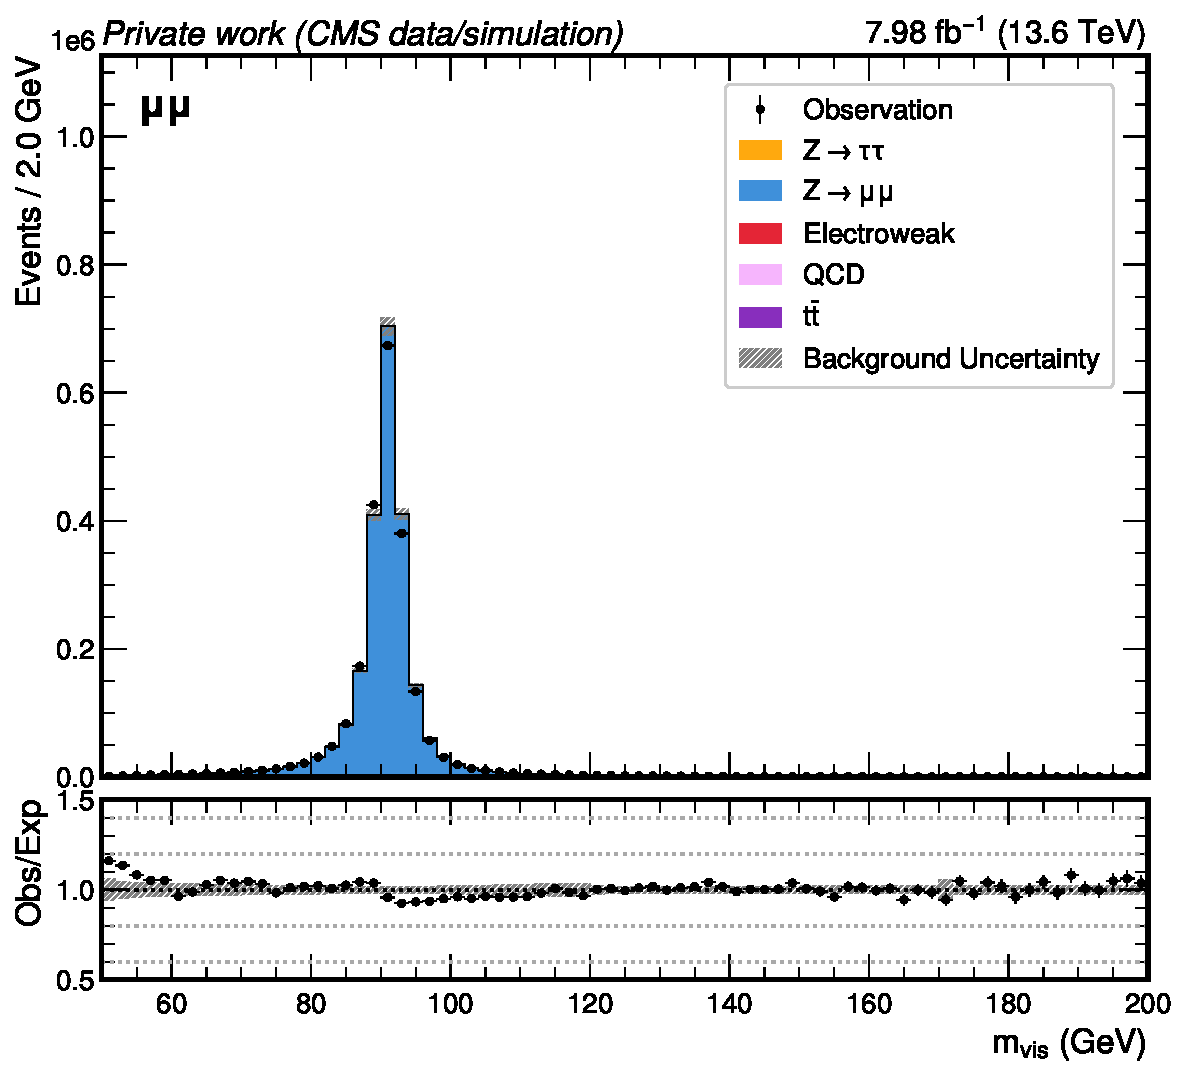
\includegraphics[width=\textwidth]{Figures/Chapter7/zpt_mvis_without.pdf}
            \caption{}
        \end{subfigure}
        \begin{subfigure}[b]{0.49\textwidth}
            \centering
            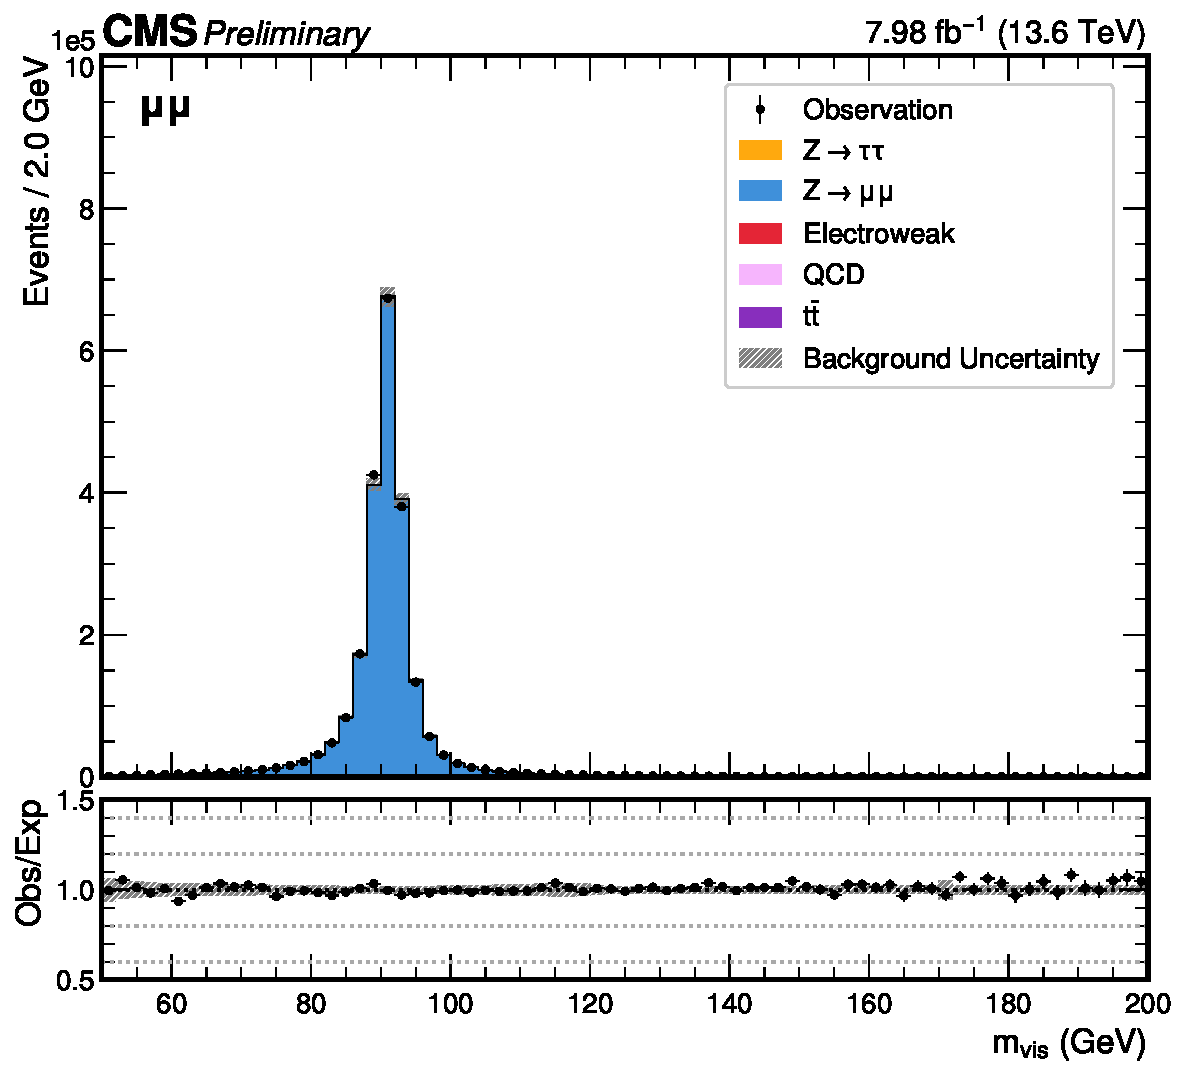
\includegraphics[width=\textwidth]{Figures/Chapter7/zpt_mvis_with.pdf}
            \caption{}
        \end{subfigure}

        \vspace{0.5cm}

        \begin{subfigure}[b]{0.49\textwidth}
            \centering
            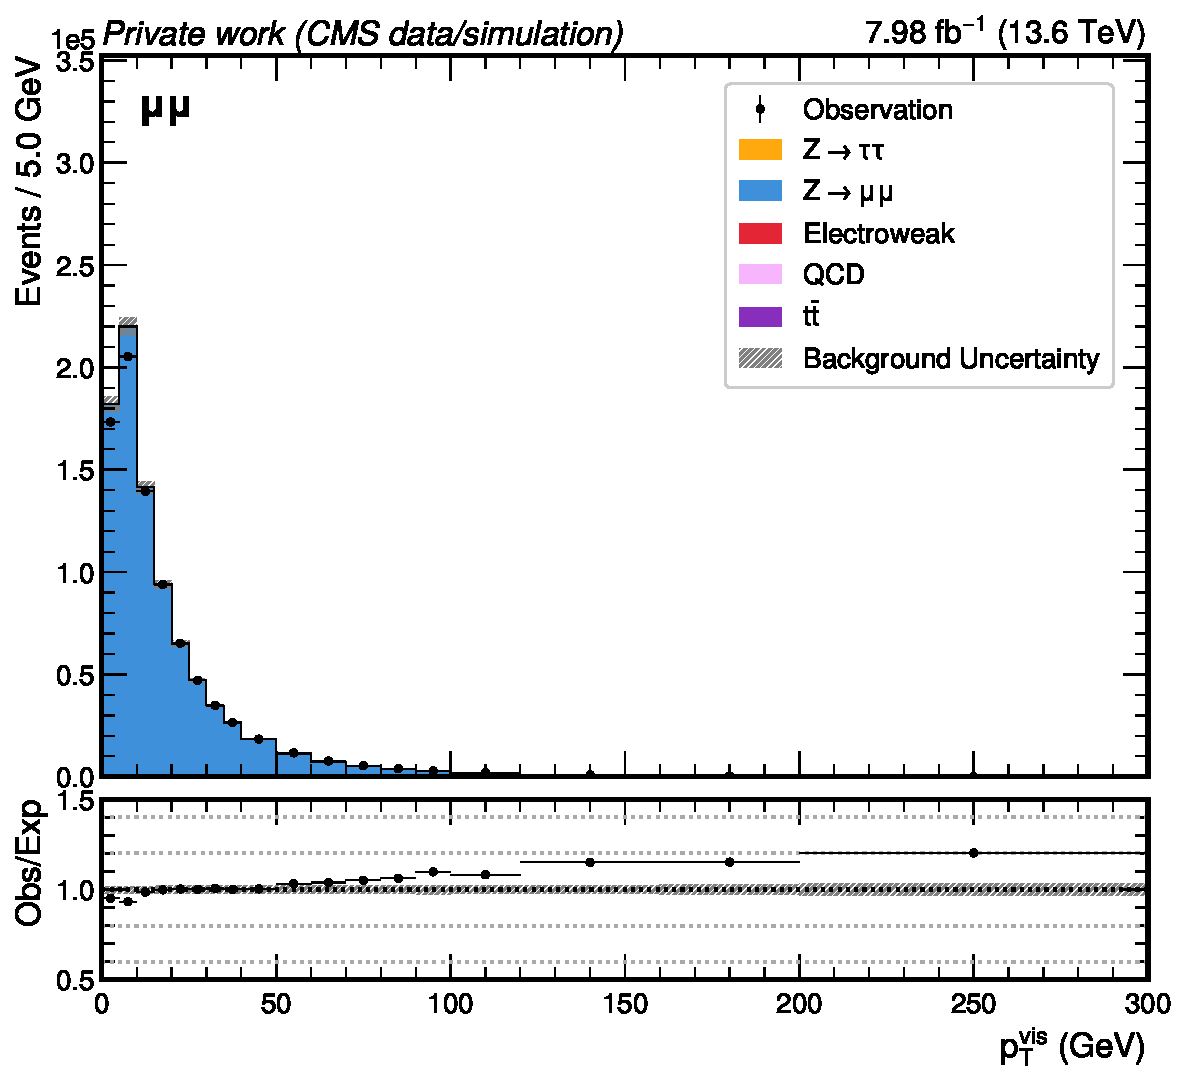
\includegraphics[width=\textwidth]{Figures/Chapter7/zpt_ptvis_without.pdf}
            \caption{}
        \end{subfigure}
        \begin{subfigure}[b]{0.49\textwidth}
            \centering
            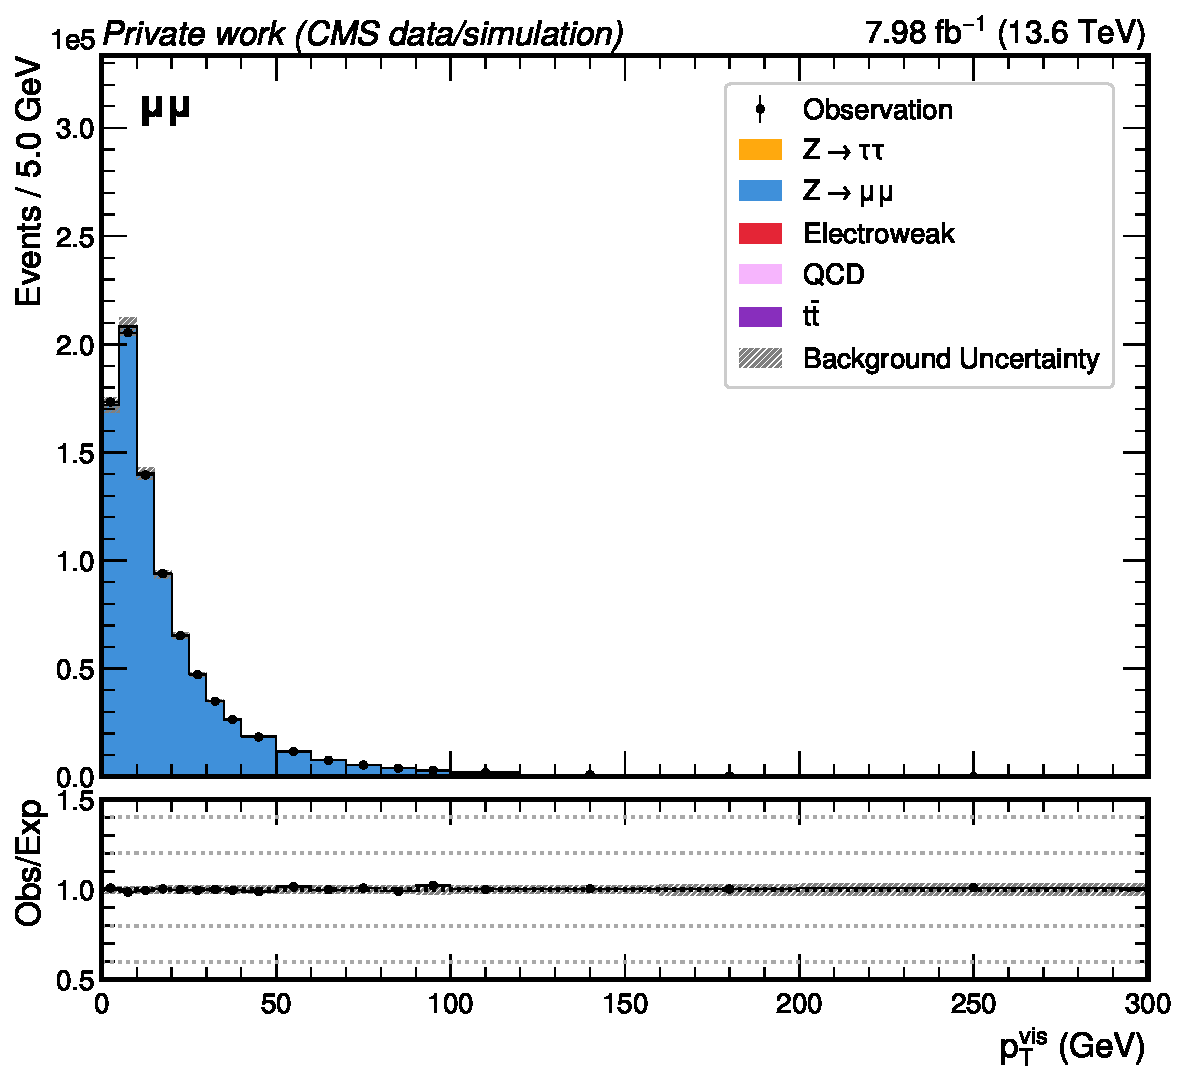
\includegraphics[width=\textwidth]{Figures/Chapter7/zpt_ptvis_with.pdf}
            \caption{}
        \end{subfigure}
    \caption[Reweighting validation in $Z/\gamma^* \to \mu\mu$ events.]{Validation of the $\PZ \, \, p_\text{T}$-mass reweighting in $Z/\gamma^* \to \mu\mu$ events. Shown are $m_\text{vis}$ distributions \textbf{(a)} before and \textbf{(b)} after reweighting, and $p_\text{T}^\text{vis}$ distributions \textbf{(c)} before and \textbf{(d)} after.}

    \label{Figure:Chapter6_ZPT_Reweighting}
\end{figure}

\begin{figure}[!htbp]
        \centering
        % First row
        \begin{subfigure}[b]{0.49\textwidth}
            \centering
            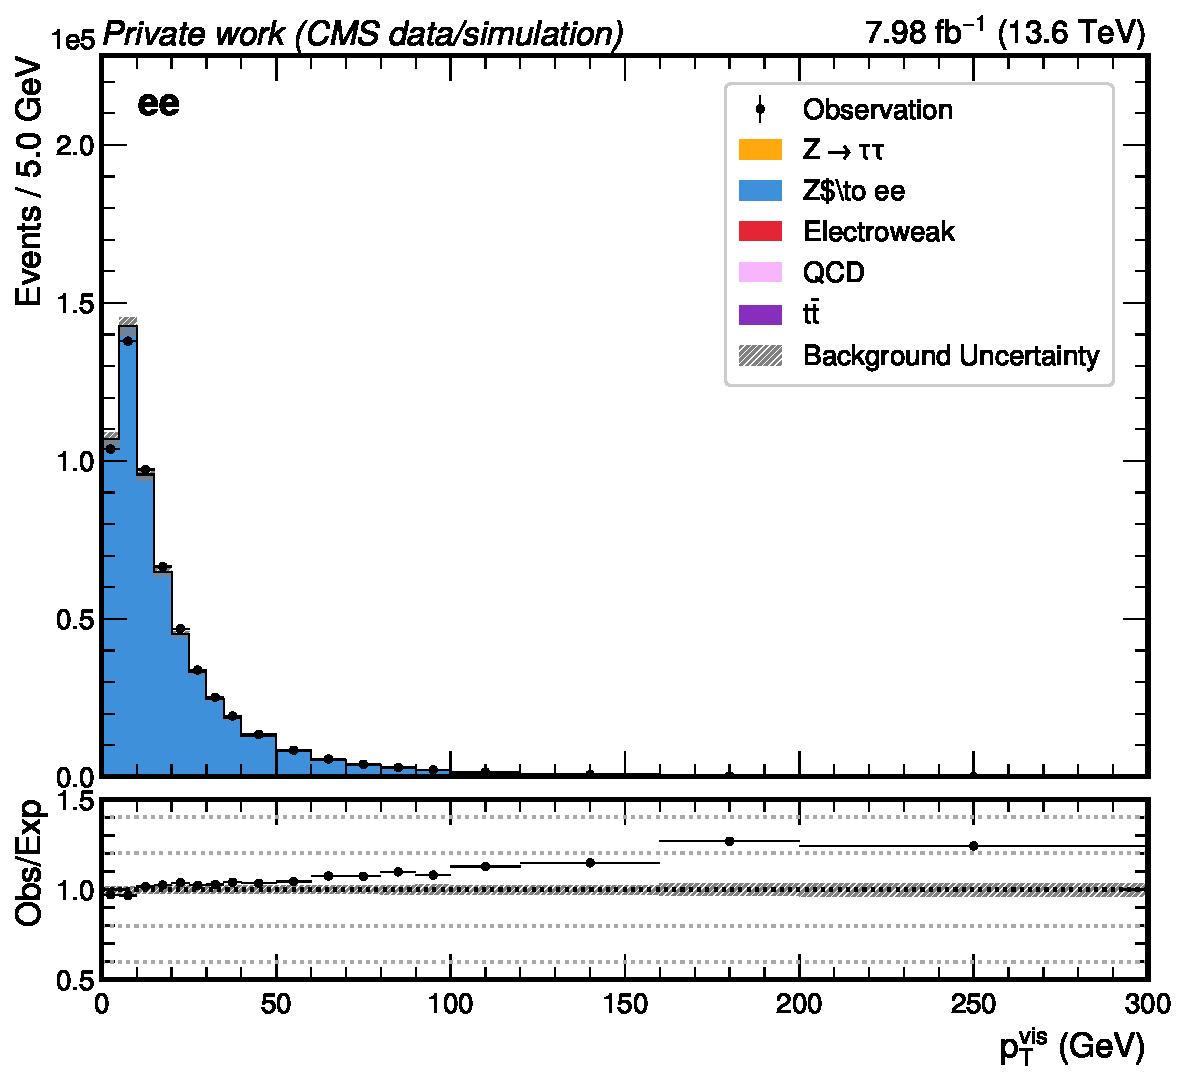
\includegraphics[width=\textwidth]{Figures/Chapter7/zpt_ee_ptvis_without.pdf}
            \caption{}
        \end{subfigure}
        \begin{subfigure}[b]{0.49\textwidth}
            \centering
            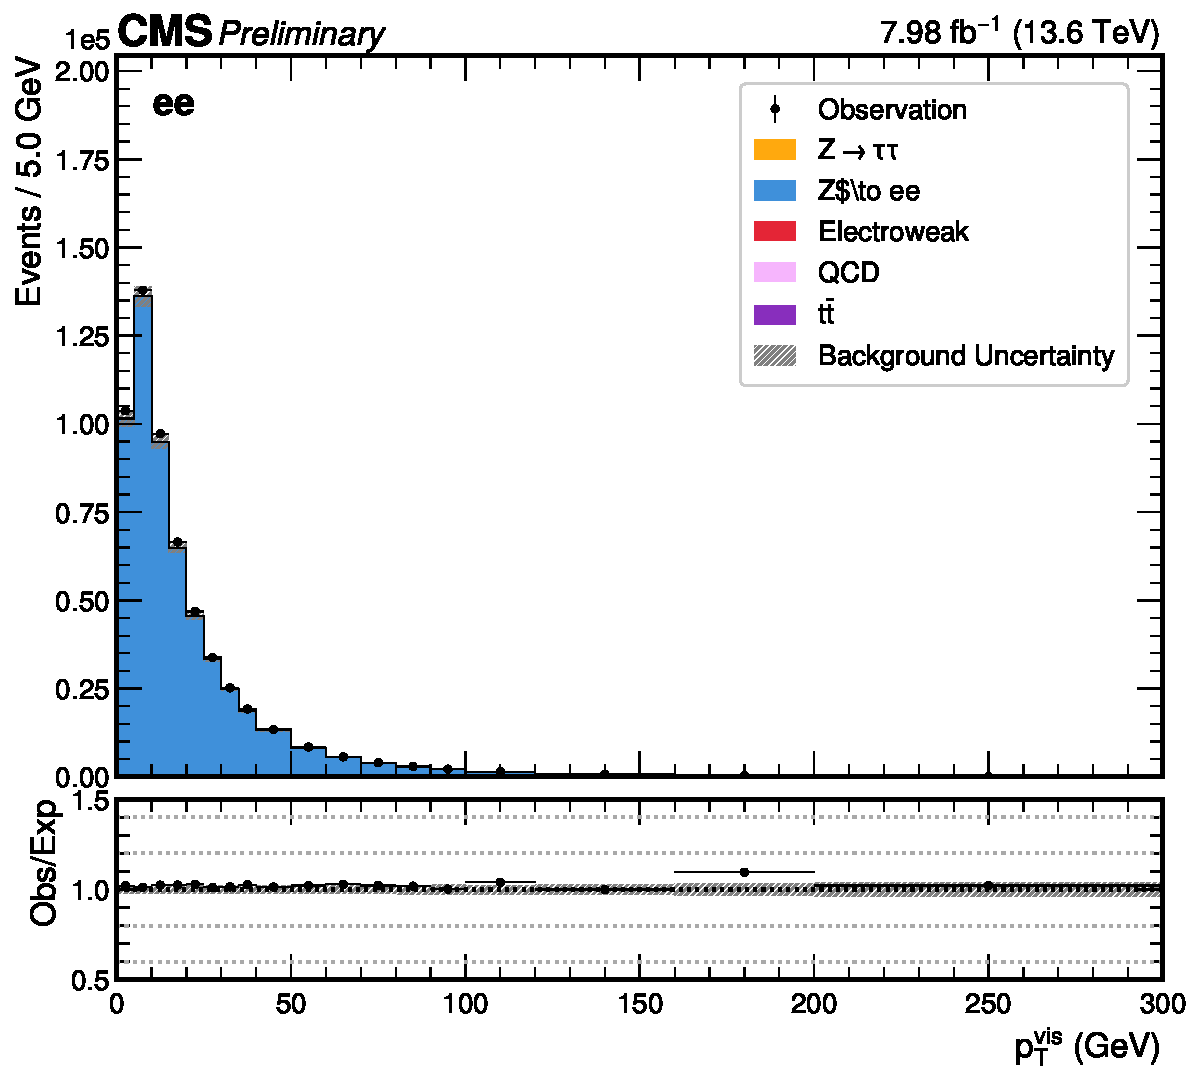
\includegraphics[width=\textwidth]{Figures/Chapter7/zpt_ee_ptvis_with.pdf}
            \caption{}
        \end{subfigure}
    \caption[Closure test of $\PZ \, \, p_\text{T}$-mass reweighting in $Z/\gamma^* \to ee$ events.]{Closure test of the $\PZ \, \, p_\text{T}$-mass reweighting in $Z/\gamma^* \to ee$ events. Distributions of $p_\text{T}^\text{vis}$ are shown \textbf{(a)} before and \textbf{(b)} after reweighting.}

    \label{Figure:Chapter6_ZPT_Reweighting_ee}
\end{figure}

\section{Background modelling}
\label{Section:Chapter7_Background_Modelling}


% Notes to Remember:
% 1. Variables not used to bias the BDT e.g. \deltaphi (differs between scenarios)